\section{Application to Quantum State Preparation}
\label{sec:applications}

% ---------------------------------------------------------------
%  OPENING: motivation and scope
% ---------------------------------------------------------------

Quantum state preparation---encoding a classical function
$f\colon \R \to \C$ into the amplitudes of a quantum
register---is a subroutine that appears across quantum
computing, from finite-element
methods~\cite{MontanaroPallister2016} and differential-equation
solvers~\cite{BerryChildsOstranderWang2017} to quantum
chemistry on grids~\cite{ChanMeisterEtAl2022} and priors for
phase estimation~\cite{BerryEtAl2022QPE}.  Efficient state
preparation is often the bottleneck of the algorithms that use it.
The standard approach requires either coherent arithmetic circuits
to construct an amplitude oracle, or a polynomial approximation
to the target function within a QSVT
pipeline~\cite{McArdleGilyenBerta2025}.  In either case, the
target function is defined on a compact interval and the output
polynomial must be bounded by~$1$ in absolute
value---restrictions that exclude functions defined on the full
real line or with unbounded range.

In this section we develop a state preparation algorithm that
exploits the stereographic framework of the preceding sections.
The central observation is that the stereographic map
$r \mapsto \rtilde = r/\sqrt{1+r^2}$ transforms the
infinite real line into the compact interval $(-1,1)$ in a way
that is compatible with QSP: rational Chebyshev expansions on
$\R$ become ordinary Chebyshev expansions in~$\rtilde$, and
Boyd's classical approximation theory~\cite{Boyd1990,Boyd1987}
provides rigorous convergence guarantees.  The resulting algorithm
handles functions defined on unbounded domains, avoids domain
truncation artifacts, and, for functions in Boyd's geometric
convergence class, achieves exponential convergence in the
polynomial degree.

The key idea is to replace the standard Chebyshev grid on a
compact interval with a \emph{cotangent grid} that covers
$(-\infty,\infty)$, and to exploit the rational Chebyshev basis
$\{\TB_k\}$ from Section~\ref{sec:main} as the natural function
space for approximation.

We seek to prepare an $N = 2^n$-dimensional quantum state whose
amplitudes encode a function $f\colon \R \to \C$:
\begin{equation}
	\ket{\Psi_f} := \frac{1}{\mathcal{N}_f}
	\sum_{j=0}^{N-1} f(y_j)\,\ket{j}, \qquad
	\mathcal{N}_f := \sqrt{\sum_j |f(y_j)|^2},
	\label{eq:target-state}
\end{equation}
where the grid points $\{y_j\}$ are determined by the
discretization scheme.

\textit{The cotangent grid.}
The stereographic map $y = L\cot\theta$ sends the interval
$\theta \in (0,\pi)$ bijectively onto
$y \in (-\infty,+\infty)$.  Taking a uniform grid in $\theta$,
we define the \emph{cotangent grid}
\begin{equation}
	y_j := L\cot\!\left(\frac{\pi(2j+1)}{2N}\right),
	\qquad j = 0, 1, \ldots, N-1,
	\label{eq:cotangent-grid}
\end{equation}
with corresponding angular grid
$\theta_j = \pi(2j+1)/(2N)$.  The half-integer shift ensures
that all $N$ grid points lie in the interior of $(0,\pi)$,
avoiding the poles of $\cot$.  The \emph{map parameter} $L > 0$
controls the density of points near $y = 0$; the effective
domain extends to $|y| \lesssim LN/\pi$, which grows
exponentially with~$n$.  This grid clusters near the origin and
becomes sparse for large $|y|$, which is dual to the Chebyshev
grid $x_j = \cos(\pi j/N)$ that clusters near $x = \pm 1$ on
the compact interval $[-1,1]$.  The cotangent grid is the
natural discretization of $\R$ for functions concentrated near
the origin with algebraic or exponential decay at infinity.

\textit{Pullback to the circle.}
Given $f\colon \R \to \C$, define its \emph{stereographic
pullback}
\begin{equation}
	g(\theta) := f(L\cot\theta), \qquad \theta \in (0,\pi).
	\label{eq:pullback}
\end{equation}
This function is precisely what a QSP circuit computes.
The connection to the rational Chebyshev basis is immediate: the
rational Chebyshev functions
$\TB_k(y;L) = \cos(k\,\mathrm{arccot}(y/L))$ and
$\SB_k(y;L) = \sin(k\,\mathrm{arccot}(y/L))$ satisfy
$\TB_k(y_j;L) = \cos(k\theta_j)$ and
$\SB_k(y_j;L) = \sin(k\theta_j)$.  Hence, a degree-$d$
rational Chebyshev approximation of $f$ on $\R$ is
\emph{exactly} a degree-$d$ trigonometric polynomial
approximation of $g$ on $(0,\pi)$, and vice versa.

\textit{Filling fraction.}
The success probability of the state preparation circuit is
governed by the \emph{filling fraction}
\begin{equation}
	\mathcal{F}_g^{[N]} := \frac{1}{\sqrt{N}} \cdot
	\frac{\bigl(\sum_{j=0}^{N-1}|g(\theta_j)|^2\bigr)^{1/2}}
	{|g|_{\max}},
	\label{eq:filling-fraction}
\end{equation}
where $|g|_{\max} := \max_{\theta \in (0,\pi)} |g(\theta)|$.
As $N \to \infty$, $\mathcal{F}_g^{[N]}$ converges to the
continuous filling fraction
$\mathcal{F}_g^{[\infty]} := \|g\|_{L^2(0,\pi)} /
(\sqrt{\pi}\,|g|_{\max})$,
which depends only on the shape of $f$ after pullback and is
\emph{independent} of any domain truncation parameter.

\textit{The Boyd class.}
The convergence rate of the rational Chebyshev expansion
determines the polynomial degree required in the QSP circuit.
We identify the relevant function class through Boyd's
classical theory~\cite{Boyd1990}: a function
$f\colon \R \to \C$ belongs to the \emph{Boyd class}
$\mathcal{B}(L)$ if $f$ is free of singularities for all
real~$y$ (except possibly at $y = \pm\infty$) and its pullback
$g(\theta) = f(L\cot\theta)$ extends to a function on
$[0,\pi]$ whose Fourier coefficients decay at an exponential
(or faster) rate,
$|a_k|, |b_k| \leq C\exp(-qk^{\rho})$ for some
$C, q > 0$ and $\rho \in (0,1]$.  Boyd's
Theorem~5~\cite{Boyd1990} identifies the analytic conditions
under which \emph{geometric} convergence ($\rho = 1$) holds:
$f$ must be analytic in a neighborhood of the real $y$-axis and
have an asymptotic power series in $1/y$ as $|y| \to \infty$
containing only nonnegative integer powers.  This class includes
Lorentzians $1/(1+y^2)^s$, hyperbolic secants, rational
functions decaying at infinity, and any function with
exponential decay.  Functions that are entire but have essential
singularities at $y = \pm\infty$---such as Gaussians---fall in
the \emph{subgeometric} class ($\rho < 1$, typically
$\rho \approx 1/2$), where the Fourier coefficients decay as
$\exp(-c\sqrt{k})$ and the required degree grows as
$d = \mathcal{O}(\log^2(1/\epsilon))$.

\textit{Algorithm.}
Our state preparation algorithm proceeds in three stages.
\emph{Stage~1 (classical preprocessing):} compute the pullback
$g(\theta) = f(L\cot\theta)$, normalize by its maximum to
obtain $\hat{g} = g/|g|_{\max}$ with $|\hat{g}| \leq 1$, and
approximate $\hat{g}$ by a degree-$d$ trigonometric polynomial
$\tilde{g}$ to $L^\infty$-error $\delta$ on $(0,\pi)$.
If $f$ has definite parity, the expansion reduces to cosines or
sines, halving the effective degree.  Compute the QSP phase
angles $\{\phi_j\}$ using standard
algorithms~\cite{DongMengWhaleyEtAl2021,Haah2019}.
\emph{Stage~2 (QSP circuit):} the signal operator is
the diagonal unitary
$e^{iA} = \sum_j e^{i\theta_j}\ket{j}\bra{j}$ with
$\theta_j = \pi(2j+1)/(2N)$.  Since $\theta_j$ decomposes
as $\theta_j = \pi/(2N) + \sum_{k=0}^{n-1} j_k \cdot \pi 2^k/N$, the
controlled signal unitary is implementable with $n$
controlled-$R_z$ gates, costing $\mathcal{O}(n)$ elementary
gates per application.  The QSP circuit uses $d$
applications of the signal unitary and its inverse, together
with $\mathcal{O}(d)$ single-qubit rotations on the ancilla.
\emph{Stage~3 (amplitude amplification):} applying the circuit
to $\ket{+}^{\otimes n}\otimes\ket{0}_a$ yields the target
state with success probability
$(\mathcal{F}_{\tilde{g}}^{[N]})^2$; we boost this to~$1$
with $\mathcal{O}(1/\mathcal{F}_{\tilde{g}}^{[N]})$ rounds of
amplitude amplification, using one additional ancilla.

\begin{theorem}[Stereographic state preparation]
	\label{thm:state-prep}
	Let $f \in \mathcal{B}(L)$ and suppose that a degree-$d_\delta$
	trigonometric polynomial approximates the normalized pullback
	$\tilde{g}(\theta) = f(L\cot\theta)/\max_\theta|f(L\cot\theta)|$
	to $L^\infty$-error
	$\delta = \varepsilon \cdot
	\min(\mathcal{F}_g^{[N]},\mathcal{F}_{\tilde{g}}^{[N]})$
	on $(0,\pi)$.  Then the algorithm above prepares a quantum state
	$\ket{\Psi_{\tilde{f}}}$ that is $\varepsilon$-close in trace
	distance to $\ket{\Psi_f}$ using
	\begin{equation}
		\mathcal{O}\!\left(
		\frac{n \cdot d_\delta}{\mathcal{F}_{\tilde{g}}^{[N]}}
		\right) \quad \text{gates},
		\label{eq:state-prep-gates}
	\end{equation}
	with at most $2$ ancilla qubits: $1$ for the QSP
	signal control and $1$ for amplitude amplification.
\end{theorem}

The proof follows the error analysis of
Ref.~\cite{McArdleGilyenBerta2025}, adapted to our setting.
For functions in the geometric convergence class ($\rho = 1$),
the degree required to achieve $L^\infty$-error $\delta$ is
$d_\delta = \mathcal{O}(\log(1/\delta)/q)$, and the total gate
complexity becomes
$\mathcal{O}(n\log(1/\varepsilon)/\mathcal{F}_g^{[\infty]})$.
For the subgeometric class ($\rho < 1$), the degree scales as
$d_\delta = \mathcal{O}((\log(1/\delta)/q)^{1/\rho})$ and the
total complexity becomes
$\mathcal{O}(n(\log(1/\varepsilon))^{1/\rho}/
\mathcal{F}_g^{[\infty]})$.

Figure~\ref{fig:convergence-comparison} illustrates these
convergence rates on four target functions, comparing the
rational Chebyshev expansion (stereographic pullback to the
circle) with standard Chebyshev approximations on truncated
domains $[-L,L]$ of increasing size.  For the Lorentzian
[panel~(a)], the rational Chebyshev expansion is exact at
degree~$2$, while the standard expansion on $[-200,200]$ has not
converged at degree~$60$.  For the hyperbolic secant and Gaussian
[panels~(b,\,c)], all methods converge, but the standard
approach degrades rapidly as the domain grows: on $[-200,200]$
even degree-$60$ polynomials fail to capture the function
accurately.  The rational Chebyshev expansion is the only method
whose convergence rate is independent of the domain size.

\begin{figure*}[tp]
	\centering
	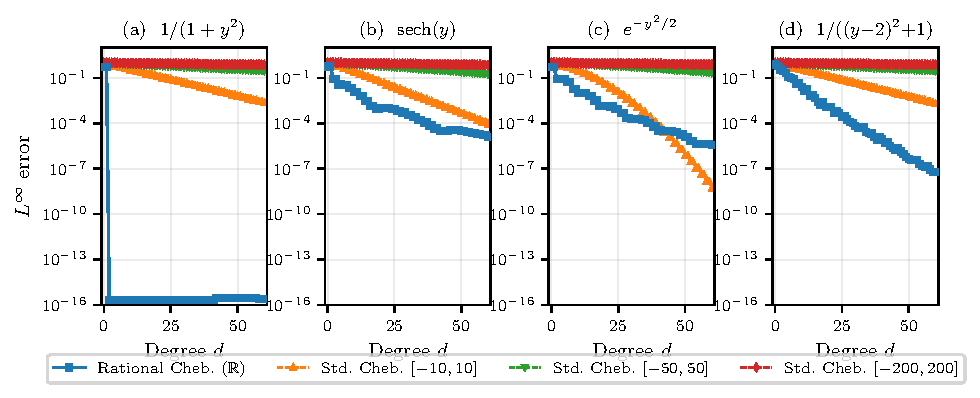
\includegraphics[width=\textwidth]{figures/convergence_comparison.pdf}
	\caption{$L^\infty$ approximation error versus polynomial
	degree~$d$ for four target functions.  Blue squares: rational
	Chebyshev expansion (stereographic pullback), which approximates
	$f$ on all of~$\R$ with no domain truncation.  Dashed lines:
	standard Chebyshev expansion on truncated domains $[-L,L]$ with
	$L = 10$~(orange), $50$~(green), and $200$~(red).
	(a)~The Lorentzian $1/(1+y^2)$ is exact at degree~$2$ in the
	rational basis, while the standard expansion degrades with~$L$.
	(b,\,c)~For sech and Gaussian targets, the standard expansion
	converges on small domains but deteriorates as $L$ grows; the
	rational Chebyshev rate is $L$-independent.
	(d)~Shifted Lorentzian: the rational expansion converges
	geometrically and outperforms the standard approach at all
	domain sizes shown.}
	\label{fig:convergence-comparison}
\end{figure*}

\textit{Lorentzian (Cauchy distribution).}
Consider $f(y) = 1/(1+y^2)$ with map parameter $L = 1$.
The pullback is
\begin{equation}
	g(\theta) = \frac{1}{1+\cot^2\theta} = \sin^2\theta
	= \frac{1-\cos(2\theta)}{2},
	\label{eq:lorentzian-pullback}
\end{equation}
a degree-$2$ trigonometric polynomial (harmonic $\cos(2\theta)$),
so $d = 2$ and \emph{no} approximation error is incurred.
The filling fraction is
$\mathcal{F}_g^{[\infty]} = \sqrt{3/8} \approx 0.612$,
a single round of amplitude amplification suffices, and
the total gate count is $\mathcal{O}(n)$.
For comparison, the method of
Ref.~\cite{McArdleGilyenBerta2025} applied to the same
function on a truncated domain $[-L,L]$ requires
approximating $h(y) = 1/(1+L^2\arcsin^2(y))$ by a
polynomial of degree
$d = \mathcal{O}(L\log(1/\epsilon))$, with filling fraction
$\mathcal{F} = \mathcal{O}(L^{-1/2})$.  For $L \sim 2^n$,
the total gate count is
$\mathcal{O}(n \cdot 2^{3n/2}\log(1/\epsilon))$---exponentially
worse.  More generally, $1/(1+y^2)^s$ pulls back to
$\sin^{2s}\theta$, a degree-$s$ trigonometric polynomial,
so the entire family of generalized Lorentzians has degree
independent of the domain size.

\textit{Hyperbolic secant.}
The function $f(y) = \operatorname{sech}(y)$ decays
exponentially, so the pullback extends smoothly to
$g(0) = g(\pi) = 0$ with all derivatives vanishing at the
endpoints.  The Fourier coefficients decay geometrically at
rate controlled by the nearest singularity of
$\operatorname{sech}(z)$ at $z = i\pi/2$, giving
$d = \mathcal{O}(\log(1/\epsilon))$ and total complexity
$\mathcal{O}(n\log(1/\epsilon))$.  This matches
Ref.~\cite{McArdleGilyenBerta2025} for $\operatorname{sech}$
on a compact domain, but handles the full real line without
truncation.

\textit{Gaussian.}
For $f(y) = \exp(-\beta y^2/2)$ with $L = 1/\sqrt{\beta}$,
the pullback $g(\theta) = \exp(-\cot^2\theta/2)$ is
$C^\infty$ on $[0,\pi]$ but has essential singularities at
the endpoints.  The Fourier coefficients decay
subgeometrically as $\exp(-c\sqrt{k})$, giving
$d = \mathcal{O}(\log^2(1/\epsilon))$ and total complexity
$\mathcal{O}(n\log^2(1/\epsilon))$.  The method of
Ref.~\cite{McArdleGilyenBerta2025} achieves
$\tilde{\mathcal{O}}(n\log^{5/4}(1/\epsilon))$ via domain
truncation---a slightly better exponent in
$\log(1/\epsilon)$, but at the cost of choosing a truncation
radius, rescaling, and composing with~$\arcsin$.

\textit{Rational functions with algebraic decay.}
Any rational function $f(y) = P(y)/Q(y)$ with
$\deg Q > \deg P$ and no real poles belongs to the geometric
convergence class.  The degree of the Fourier approximation is
controlled by the distance of the nearest complex pole from the
real axis.  For example, $f(y) = 1/((y-a)^2+b^2)$ with
$b > 0$ requires degree
$d = \mathcal{O}(L/b \cdot \log(1/\epsilon))$ in general;
when centered ($a = 0$) with natural width ($b = L$), this
reduces to $d = \mathcal{O}(\log(1/\epsilon))$, independent
of~$L$.  Table~\ref{tab:state-prep-comparison} collects the
gate complexity for all four targets.

\begin{table}[t]
	\caption{Gate complexity for state preparation of target
	functions on unbounded domains.  Here $n$ is the number of
	qubits, $\varepsilon$ the target trace distance, and
	$L \sim 2^n$ the domain truncation parameter for the
	standard approach.  The stereographic approach requires no
	domain truncation.}
	\label{tab:state-prep-comparison}
	\begin{ruledtabular}
		\begin{tabular}{lll}
			Target $f(y)$
			 & Standard~\cite{McArdleGilyenBerta2025}
			 & Stereographic                                            \\
			\hline
			$1/(1+y^2)$
			 & $\mathcal{O}(n\cdot 2^{3n/2}\log\frac{1}{\varepsilon})$
			 & $\mathcal{O}(n)$                                         \\[4pt]
			$\operatorname{sech}(y)$
			 & $\mathcal{O}(n\log\frac{1}{\varepsilon})$
			 & $\mathcal{O}(n\log\frac{1}{\varepsilon})$                \\[4pt]
			$e^{-\beta y^2/2}$
			 & $\tilde{\mathcal{O}}(n\log^{5/4}\frac{1}{\varepsilon})$
			 & $\mathcal{O}(n\log^2\frac{1}{\varepsilon})$              \\[4pt]
			$\frac{1}{(y-a)^2+b^2}$
			 & $\mathcal{O}(\frac{nL}{b}\log\frac{1}{\varepsilon})$
			 & $\mathcal{O}(\frac{nL}{b}\log\frac{1}{\varepsilon})$
		\end{tabular}
	\end{ruledtabular}
\end{table}

The key structural differences between the stereographic and
standard approaches are threefold.  First, the domain: the
stereographic method works on $(-\infty,\infty)$ via the
cotangent grid, while the standard method requires a finite
domain $[-L,L]$ whose size must grow with~$n$.  For functions
with algebraic decay, this distinction is decisive---the domain
truncation introduces both Gibbs artifacts and an exponentially
growing gate count.  Second, the approximation basis: rational
Chebyshev functions can convert a non-polynomial target like
$1/(1+y^2)$ into an exact low-degree polynomial
$1 - \rtilde^2$, while the arcsine substitution has no
comparable simplification.  Third, the two approaches share the
same circuit template and ancilla count ($\leq 2$ qubits),
differing only in the classical preprocessing and the function
space used for approximation.
